\documentclass[a4paper]{book}

% Load the VUB package.
% This has many options, please read the documentation at
% https://gitlab.com/rubdos/texlive-vub
\usepackage{vub}
\usepackage{booktabs}
\usepackage{graphicx}
\usepackage{listings}
\usepackage{caption}
\usepackage{xcolor}
\graphicspath{ {./images/} }

%\captionsetup[figure]{position=bottom}
%\captionsetup[listings]{position=bottom}


% Some highly suggested packages, please read their manuals.
%\usepackage{cleveref}
\usepackage[natbib,style=apa]{biblatex}
\addbibresource{references.bib}

\title{Distributing first-class reactors in a cluster environment}
\pretitle{\flushleft{Graduation thesis submitted in partial fulfilment of the requirements for the degree of de Ingenieurswetenschappen: Applied informatics}}
%\subtitle{Haai Virtual machine}
\author{Hans Van der Ougstraete}
\date{June~2024}
\promotors{Promotors: prof.\ dr.\ Wolfgang De Meuter,\and prof.\ dr.\ Joeri De Koster \and Supervisor: Bjarno Oeyen}

\faculty{sciences and bioengineering sciences} % Note: without the word "Faculty"!

\begin{document}
\frontmatter
\maketitle%

% Oftentimes, you need add a second language title.
\title{Distributing first-class reactors in a cluster environment}
\pretitle{\flushleft{Proefschrift ingediend met het oog op het behalen van de graad van Master of Science in de Ingenieurswetenschappen: Toegepaste informatica}}%
%\subtitle{mijn ondertitel}
\date{Juni~2024}%
\promotors{Promotors: prof.\ dr.\ Wolfgang De Meuter, \and prof.\ dr.\ Joeri De Koster \and Supervisor: Bjarno Oeyen}
\faculty{wetenschappen en bio-ingenieurswetenschappen}%
\maketitle%

\chapter{Abstract}
Reactive programming has gained significant traction for its efficacy in handling asynchronous and event-driven scenarios, particularly in distributed systems. This paradigm emphasizes responsiveness, scalability, and resilience, making it an ideal choice for real-time applications. However, distributing reactive programming introduces challenges such as consistency, coordination, fault tolerance, and communication overhead. This thesis investigates these challenges and proposes a system designed to address them. By leveraging a shared-nothing architecture and deploying an Erlang cluster, we develop a runtime for the purely functional reactive language Haai. This system aims to eliminate known issues in distributed reactive programming, such as the Reactive Thread Hijacking Problem and Reactive/Imperative Impedance Mismatch. We detail the implementation of the Haai virtual machine (Hvm), the deployment of reactors, and the management of distributed environments to enhance scalability, fault tolerance, and performance in distributed reactive systems.

\tableofcontents%

\mainmatter%
\chapter{Introduction}

Reactive programming has been around for a while, gaining traction in various domains due to its ability to handle asynchronous and event-driven scenarios effectively. One of its notable advantages lies in its suitability for distributed systems. By its nature, reactive programming facilitates the development of systems that can easily scale across distributed environments, allowing components to communicate asynchronously and react to events in real-time. However, distributing reactive programming poses several challenges (\cite{DBLP:journals/csur/BainomugishaCCMM13}) such as consistency, coordination, fault tolerance and many more. These challenges highlight the need for further research and study in understanding how reactive programming principles can be effectively applied and scaled in distributed environments. By investigating these challenges, we can gain insights into best practices and architectural approaches for building robust and scalable distributed reactive systems.

\section{Reactive programming} \label{sec:irp}
Reactive Programming (RP) is a broader programming paradigm that encompasses the idea of reacting to changes and events in a system. It involves modeling the flow of data as streams of events and using declarative and composable abstractions to handle asynchronous and event-driven scenarios. The canonical reactive program model (ref?) is based on time-varying values and propagation of change. 

Spreadsheets offer a good example to illustrate this. When a cell containing a formula that includes other cells it is dependent on the cells that are used in that formula. As an example lets take a cell A3 that contains the formula "=A1*A2" whenever the value changes in the cells A1 or A2, A3 will automatically update. We call each spreadsheet cell a time-varying value or signal because there concrete value changes over time due to events. In this example, an event could be when a user changes the value A1 or A2 using the gui of the spreadsheet program.

The two fundamental abstractions defined by RP to represent time-varying values are behaviors and events. Both can be seen as time-varying values but behaviors are said to be continuous over time whilst events are discrete over time. Behaviors have a value at any moment (continuous). Events have a value at specific moments in time (discrete). 
Listing \ref{code:Haairp} shows the spreadsheet example represented in the RP language Haai (\cite{oeyen_reactive_2024}).
In this example A3 is defined as a behavior that continuously contains the result of a1 * a2. For each time that an event occurs updating a1 or a2, A3 will be automatically updated. One could say that the tempo or rhythm of the propagation of change for the behavior A3 depends on the speed that events have a new discrete value.     
\begin{lstlisting}[language=C, caption={Haai code}, captionpos=b, label={code:Haairp}, basicstyle=\ttfamily, frame=single]
	(defr (A3 a1 a2)
	(out (* a1 a2)))
\end{lstlisting}


\section{Problem Statement}
The distribution of reactive programming (RP) introduces a myriad of complexities and challenges. In this work we would like to focus on the following two challenges. Developing a declarative specification to deploy the distributed reactive program and simulating a virtual general clock between the individual nodes by temporizing the occurrence of events or discrete time-varying values.  

\section{Overview}
The Structure of this thesis starts with a situation of (distributed) reactive programming. After explaining the strategy of the thesis we explain purely reactive programming in section \ref{sec:prp}. More detail on the runtime is found in chapter \ref{sec:Hvm}. Chapter \ref{sec:distribution} explains the distribution of the runtime and the tools used to build it. Before ending with the conclusion we have chapter \ref{sec:evaluation} with the evaluation of the distribution and the musical use case of the distributed reactive melody generator. 

\section{Strategy and Methodology}

In order to run the first-class reactors in a distributed setting we setup a cluster environment. The cluster environment is build as a shared nothing architecture (sna) and hosts an Erlang cluster. We have chosen this architecture for basic simplicity as it allows to easily scale and monitor fault tolerance since each node is independent and self-sufficient.

To deploy the system (combination of firs-class reactors) we make use a declarative domain specific language to define which reactor needs to run on what node or group of nodes. We have build a runtime for the purely functional reactive language Haai on top of the sna. Each node represents a runtime towards which a (master) node can send the code to be deployed.

All the different nodes or runtimes in the cluster have a rhythmical organization (eg: the loop time of a reactor is a fixed value in milliseconds).   

\chapter{Reactive programming}

Reactive programming (RP) and reactive streams (RS) are terms that are often used interchangeably. Both adhere to the same canonical model, explained in section \ref{sec:irp}, showing there similarities. Two fundamental differences instead are the way dependencies between signals are established and how updates to signals are orchestrated.

\subsubsection{Signal Dependencies}
The way signal dependencies are established in the source code differs in the following way. In RP languages these dependencies are automatically taken care of by the language. Programmers implement there desired functionality in RP similar as they would in a non-reactive language. In RS the dependencies are explicitly programmed by the programmer by making use of operators provided by the RS library. The programmer creates a linear application of those operators often called a pipe as shown in listing \ref{code:rxpy} where an observable exiting of the numbers 1 to 10 will be the source of the pipe. The second or last operator in the pipe is Sum, who will produce one value to be printed on screen.

\subsubsection{Signal Orchestration}
The operators used in RS define independently for each signal how these will be updated. In contrary to RP where it is again the system that updates signals in a global way. As can be seen in listing \ref{code:Haairp}, no special code defines how or in what order the values a1 and a2 need to be updated. Both approaches can fail and result in a glitch, if for example the RP language updates signals in the wrong order, dependent signals end up having the wrong value, this is called a glitch. On the other hand in RS, if the programmer does not exactly know what an operator does and uses it in a pipe or collection of operators, inconsistencies might arise and also produce a glitch. 

\vspace{1em} % Adjust the space as needed
\noindent
The responsibility to handle signal dependencies and orchestration correct is at the system side for RP and in the developers hand for RS.


\begin{lstlisting}[language=Python, caption={Python, RxPy library},captionpos=b, label={code:rxpy}, basicstyle=\small\ttfamily, frame=single]
rx.of(1,2,3,4,5,6,7,8,9,10).pipe(
	operators.filter(lambda i: i %2 == 0),
	operators.sum()
).subscribe(lambda x: print("Value is {0}".format(x)))
\end{lstlisting}


\section{State of the art}

In this section and the rest of this thesis we will focus on reactive programming. Reactive programming has many applications we will show tree selected examples. Fran (\cite{DBLP:conf/icfp/ElliottH97}) the first reactive programming language, originated to compose interactive multimedia animations based on behaviors and events. Listing \ref{code:fran} show a small fran code example that animates a bitmap file with the moveXY behavior given the argument wiggle (a value that changes over time form 0 to +1 to -1 back to 0 and so on) for x and 0 for y.
\begin{lstlisting}[language=Python, caption={Fran, animation},captionpos=b, label={code:fran}, basicstyle=\small\ttfamily, frame=single]
leftRightCharlotte = moveXY wiggle 0 charlotte
charlotte = importBitmap "../Media/charlotte.bmp"
\end{lstlisting}

ReactiFi (\cite{DBLP:journals/programming/SterzEMBGHMF21}) a high-level reactive programming language to program Wi-Fi chips on mobile consumer devices without expert knowledge of Wi-Fi chips. In listing \ref{code:reactifi} we show part of the code for adaptive file sharing programmed on the Wi-Fi chip. A ReactiFi program exists out of reactives, like monitor, frames en count in the example, that are reactive definitions of individual processing steps triggered by incoming events.

\begin{lstlisting}[language=Python, caption={ReactiFi, Wi-Fi file sharing},captionpos=b, label={code:reactifi}, basicstyle=\small\ttfamily, frame=single]
 val monitor = Source(Monitor)
 val frames  = monitor.filter(frame -> { frame.dst == ADDR })
 val count   = frames.fold({ 0 })((count, frame) -> { count + 1 })
\end{lstlisting}

The domain-specific language Yampa (\cite{DBLP:conf/haskell/CourtneyNP03}) embedded in Haskell for programming hybrid (mixed discrete-time and continuous-time) systems. Listening \ref{code:yampa} shows a signal function that describes the behavior of a bouncing ball with position (p) and velocity (v) that are continuously updated over time. When the discrete event 'hitGround' occurs the velocity of the ball reverses.
\begin{lstlisting}[language=Python, caption={Yampa, bouncing ball},captionpos=b, label={code:yampa}, basicstyle=\small\ttfamily, frame=single]
-- The bouncing ball signal function
fallingBall :: SF () Ball
fallingBall = proc () -> do
 rec
   -- Velocity integrates to position
   v <- integral -< gravity
   p <- integral -< v

   -- Event that occurs when the ball hits the ground
   let hitGround = if p <= 0 then Event () else NoEvent
	
   -- Velocity changes direction on hit
   v <- (arr (\v -> if p <= 0 then -v else v) <<< identity) -< v

 returnA -< (p, v)
\end{lstlisting}


Most, if not all, of the reactive programming languages are build on top of a sequential host language. Fran and Yampa are build on Haskell, ReactiFi is build on Scala and C. This allows the reactive programming languages to leverage the existing ecosystems of the host language. For example a host languages can provide functions to be called form the reactive programming language, this is called lifting, the host-functionality is lifted form the host language into the RP language adapted to work with continuous and discrete notions of time. On the other hand, when a system is composed of those two components, the host part and the reactive part, they are prone to the \textit{Reactive Thread Hijacking Problem} and the \textit{Reactive/Imperative Impedance Mismatch} problems (\cite{vonder_tackling_2020}). Both problems could make stop a reactive program from being reactive. In section \ref{sec:prp} we will introduce a novel reactive language Haai that by design excludes both problems mentioned above.  



\section{Distributed reactive programming} \label{sec:drp}


Different distributed systems can be thought of as a reactive system. The distributed system reacts to events in a similar way a non distributed reactive system would do. For example an internet of things application with many connected sensors. Or a distributed reactive system with strong computational differences for different behaviors that should finish in a certain requested time. The distribution can optimize multiple nodes with different computational capacities related to the application. 

Once working in a distributed setting, typical problems arise like data inconsistencies and node disconnects and crashes. In the literature inconsistencies in the data are called glitches. A glitch is a momentary inconsistency in a time-varying value. For example in a financial application we do not want to read inconsistent values. We need to be sure that all dependencies for a certain value are correct before reading that value. Being free of glitches is called glitch-freedom (\cite{DBLP:journals/tse/MargaraS18}). 

To date, REScala has been the only reactive language providing a solution to node disconnects and crashes in distributed reactive programs. REScala does not delegate the responsibility to handle errors to the host language (Scala). REScala has been extended to support recovery after node crashes and cope with unreliable network connections by enhancing the data flow graph for a particular program (\cite{DBLP:conf/ecoop/MogkBSFM18}). Listing \ref{code:rescala} shows a shared calendar application written in REScala. This is a distributed application where one calendar is shared among many users. In order to provide recovery after crashes, signals such as Var[Date] are stored in snapshots. This allows for the signal to be reloaded after a crash. In cases where a signal is dependent on dynamic signals in the network of distribution, the REScala program handles errors explicitly. For example the selectedEntries in code listing \ref{code:rescala} expects a value from another node (selectedWeek.value). The try catch block will by default wait for the value but by returning false in the catch block the filter will drop this signal and continue filtering when a 'disconnectedSignal' error is received. By doing so the program does not block and keeps on running reactively.  

\begin{lstlisting}[language=Scala, caption={REScala, shared calendar application},captionpos=b, label={code:rescala}, basicstyle=\small\ttfamily, frame=single]
val newEntry = Evt[Entry]()
val automaticEntries: Event[Entry] = App.nationalHolidays() 
val allEntries = newEntry || automaticEntries 

val selectedDay: Var[Date] = Var(Date.today) 
val selectedWeek = Signal { Week.of(selectedDay.value) } 

val entrySet: Signal[Set[Entry]] = 
 if (distribute) ReplicatedSet("SharedEntries").collect(allEntries)
 else allEntries.fold(Set.empty) { (entries, entry) => entries + entry}

case class Entry(title: Signal[String], date: Signal[Date]) 

val selectedEntries = Signal {
 entrySet.value.filter { entry => 
 	try selectedWeek.value == Week.of(entry.date.value)
 	catch { case DisconnectedSignal => false } 
 } 
} 

allEntries.observe(Log.appendEntry)
selectedEntries.observe(
 onValue = Ui.displayEntryList, 
 onError = Ui.displayError)
\end{lstlisting}


\section{Purely reactive programming} \label{sec:prp}
In all previous examples the reactive programming language is build on top of a host language that lend some functionality to the reactive program. What we will discuss next is the idea of a purely reactive program. A reactive program constructed by combining only reactive programs that we call reactors.
\subsection{Reactors}
In Haai, a purely reactive computer language, the only construct available for expressing computations is a reactor. A reactor is a sort of blue print (as shown in figure \ref{fig:reactor}) that will be used to deploy any number of deployments based on that reactor. We can write a single reactor or combine multiple reactors in one 'main' reactor or program. The main program is build out of reactors, these can be native or user defined. Every computation in a reactor is done by a reactor, some are native to the runtime others are user defined. For example the runtime could provide native reactors for basic arithmetic. All functionality in the purely reactive programming language Haai comes from the language itself, it is not build on top of a host language. 

\begin{figure}[h]
	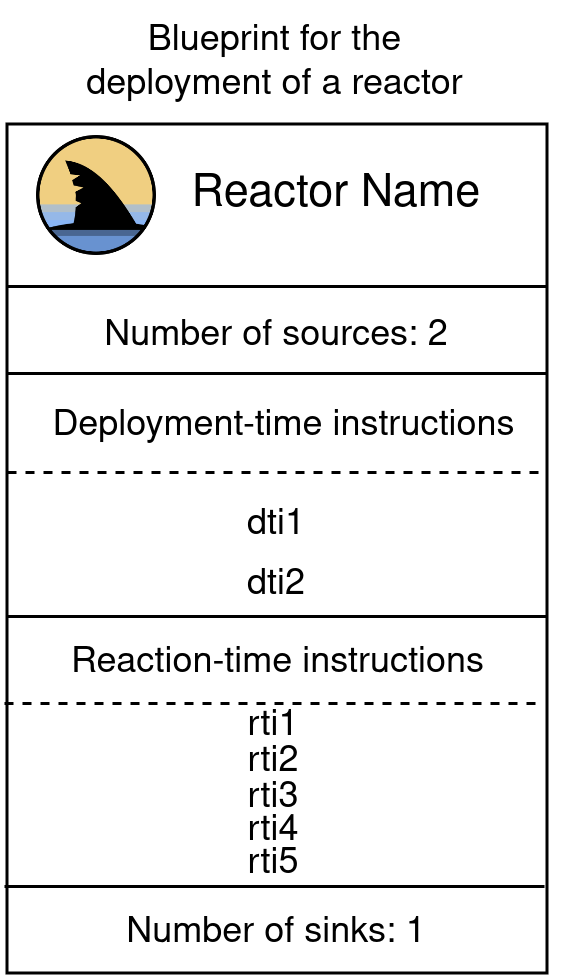
\includegraphics[scale=0.2]{reactor300.drawio}
	\centering
	\caption{Graphical representation of a reactor}
	\label{fig:reactor}
\end{figure}

The deployment of a reactor reacts on a data stream, that data altered by the reaction is found in the sink of the reactor. The deployment of a reactor is further explained in section \ref{sec:dar}.

\subsection{Haai}
We are making use of the novel purely reactive language Haai. Haai is reactive all-the-way-trough. As such the only construct available for expressing computations is a reactor. A reactor has sources or inputs and sinks or outputs. For each time the sources are updated the reactor will react and produce a new sink value. The number of sources and sinks are variable per reactor definition. In Haai there are no functions, only reactors. This allows us to build reactive programs without functions (\cite{oeyen_reactive_2024}). Haai is an independent language, it does not work on top of a host-language.  

\subsubsection*{Haai Code example}
This Haai code in listing \ref{code:Haai} represents three user defined reactors: consonance, duration and main. The main reactor is build out of the two user defined reactors consonance and duration and makes no use of native reactors (except for the ones in consonance and duration). Consonance and duration make use of multiple native reactors to perform arithmetic. The arguments to the reactor are the sources and the keyword 'out' defines the sink of the reactor.

\begin{lstlisting}[language=C, caption={Haai code}, captionpos=b,label={code:Haai}, basicstyle=\ttfamily, frame=single]
(defr (consonance f)
	(out (* ci f)))

(defr (duration bpm)
	(def q (/ 60000 bpm))
	(out (* lm q)))

(defr (main f bpm)
	(out (consonance f))
	(out (note_length bpm)))
	
\end{lstlisting}
The reactor in listing \ref{code:Haai} has two sources (f and bpm) and two sinks defined with the keyword out. To port the Haai code (listing \ref{code:Haai}) into the cluster environment we compile the Haai code into a byte code representation (listing \ref{code:bytecode}) that was developed for the Remus virtual machine. "a virtual machine that has been carefully designed to be usable for running reactive programs in low-powered computing environments."(\cite{oeyen_remus_2022})


\subsection*{Remus instruction set}
The Remus instruction set in table \ref{tab:instructionset} is the set of low-level operations that the virtual machine can execute. A Haai program or Reactor will after compilation exist out of a combination of instructions. Instructions form the Remus instruction set as listed here under. The Haai virtual machine is an implementation of this instruction set in Elixir. The following example program is build up out of a combination of the Remus instruction set. It is the compilation of the main reactor shown in the code snippet above. 

\begin{table}[h!]
	\centering
	\begin{tabular}{@{}lll@{}}
		\toprule
		\textbf{Instruction} & \textbf{Arguments} & \textbf{Description} \\ \midrule
		I-ALLOCMONO & [reactor]  & Allocate memory for the given reactor. \\
		I-LOOKUP & [signal]  & Lookup the value for signal \\
		I-SUPPLY & [from, destination, index] &  Move a value.\\
		I-REACT  &[memory\_location] & Apply the reaction found in memory. \\
		I-CONSUME & [memory\_location, index] & Position the result of react in run-time-memory. \\
		I-SINK & [rti\_location, sink\_index]& Position a value from run-time-memory into sink. \\ 
		\toprule
	\end{tabular}
	\caption{Remus instruction Set}
	\label{tab:instructionset}
\end{table}

\subsubsection*{Bytecode example}

After parsing the bytecode that was compiled form the original Haai code in listing \ref{code:Haai} with the Remus compiler into an Elixir readable format of nested lists a program looks like listing \ref{code:bytecode}. In this example we see two user defined reactors named consonance and note\_length followed by the main reactor with 2 sources and 2 sinks that represents the actual program that will be deployed in the cluster environment.

\begin{lstlisting}[language=C, caption={Remus bytecode as Elixir nested lists},captionpos=b, label={code:bytecode}, basicstyle=\ttfamily, frame=single]
[
 [:consonance, 1, 1,
	[
		["I-ALLOCMONO", :multiply]
	],
	[
		["I-LOOKUP", :ci],
		["I-SUPPLY",["%RREF",1],["%DREF",1],1],
		["I-SUPPLY",["%SRC",1],["%DREF",1],2],
		["I-REACT",["%DREF",1]],
		["I-CONSUME",["%DREF",1],1],
		["I-SINK",["%RREF",5],1]]
	],

 [:duration, 1, 1,
	[
		["I-ALLOCMONO", :divide],
		["I-ALLOCMONO", :multiply]
	],
	[
		["I-SUPPLY",60000,["%DREF",1],1],
		["I-SUPPLY",["%SRC",1],["%DREF",1],2],
		["I-REACT",["%DREF",1]],
		["I-LOOKUP",:lm],
		["I-SUPPLY",["%RREF",4],["%DREF",2],1],
		["I-CONSUME",["%DREF",1],1],
		["I-SUPPLY",["%RREF",6],["%DREF",2],2],
		["I-REACT",["%DREF",2]],
		["I-CONSUME",["%DREF",2],1],
		["I-SINK",["%RREF",9],1]]
	],

 [:main, 2, 2,
	[
		["I-ALLOCMONO", :consonance],
		["I-ALLOCMONO", :note_length]
	],
	[
		["I-SUPPLY",["%SRC",1],["%DREF",1],1],
		["I-REACT",["%DREF",1]],
		["I-SUPPLY",["%SRC",2],["%DREF",2],1],
		["I-REACT",["%DREF",2]],
		["I-CONSUME",["%DREF",1],1],
		["I-SINK",["%RREF",5],1],
		["I-CONSUME",["%DREF",2],1],
		["I-SINK",["%RREF",7],2]
	]
 ]
]
\end{lstlisting}

\section{Haai virtual machine} \label{sec:Hvm}
To run the Haai code or compiled bytecode we implement in this thesis a virtual machine for Haai. The purpose of the Haai virtual machine (Hvm) is to enable the distribution of first-class reactor Haai programs in a cluster environment. The Hvm is developed in Elixir, a computer language know for its powerful features in terms of distribution and concurrency. It leverages the Erlang Virtual Machine (BEAM), which is renowned for its ability to build scalable, fault-tolerant, and distributed systems (\cite{10.5555/1951582}).

\subsection{Deploying a reactor} \label{sec:dar}
A reactor can be seen as a blue print for its deployment, similar to how an object created from a class in object-oriented programming is an instantiation of the blueprint that the class represents. The deployment of the reactor will request a certain size of memory. 
That total block of memory (shown in figure \ref{fig:rde}) exists out of four parts: sources, deployment time memory (dtm), reaction time memory (rtm) and the sinks. 

When we go from a reactor to a deployment we can find the following information in the reactor or blue print for the deployment. The number of sources and sinks, the deployment time instructions (dti) and the reaction time instructions (rti). For each source and each sink a position is reserved in the memory block we are constructing. From the deployment time instructions in the reactor we can prepare the deployment time memory (dtm). The Dtm part of the memory block we are constructing will reserve space for the deployment of the reactors found in the dti. 

Sofar the space for the sources, the sinks and dtm has been reserved, the last step is to reserve space for the reaction time memory (rtm). The space required for rtm is equal to the number of instructions found in the reaction time instructions. For each instruction in rti there is one block reserved in rtm. A deployed reactor uses the four memory parts: sources, dtm, rtm and sinks to react according to the reaction time instructions found in rti.

\begin{figure}[h]
	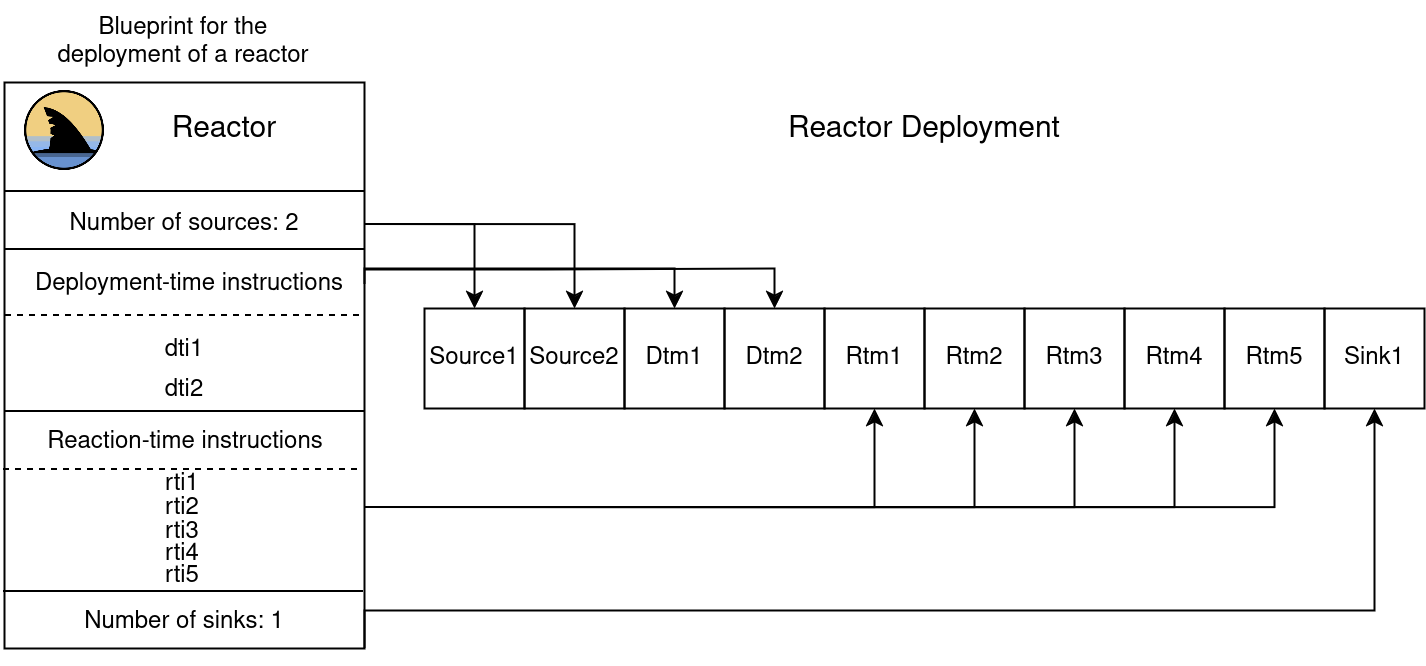
\includegraphics[width=\textwidth]{rd.drawio}
	\caption{Reactor deployment, from blueprint to memory block}
	\label{fig:rde}
\end{figure} 

\subsection{Starting the deployment}
The deployment needs to be its sources and sinks to the runtime in order to communicate with the system. Sources are connected to a function that call's the next value for the sources after each iteration of the deployed reactor. Similarly the sinks are connected to a function that given the values of the sink handles them in the required way for the overall program. Section \ref{sec:evaluation} presents a musical use case where the values found in the sink serve as values for OSC messages.


\subsection{Managing the reactors state}
Managing the state of a reactor is handled by a single actor per program or reactor deployment. This actor is built around the GenServer module in Elixir, a behavior module that provides a generic server implementation. In this implementation, the GenServer is named Memory. Memory serves as a single actor that encapsulates multiple functions designed to respond to various messages or calls. These functions collectively define the behavior of the Memory GenServer.

Memory primarily accepts calls from the runtime instructions found in the reactor deployment. These calls are mapped to the Haai instruction set. Additionally, there are calls to initialize the Memory GenServer, as well as to get or set sources and sinks within it. One instance of Memory represents the memory block of a deployed reactor.

The GenServer module in Elixir operates with calls or casts. In this context, we use calls, which are synchronous requests to the GenServer. By making synchronous calls to Memory, we ensure that the values within Memory are accessed by only one operation at a time, thereby maintaining the integrity and correctness of these values.

\subsection{Native reactors}
The Haai virtual machine makes use of native reactors to perform simple arithmetic operations like addition, division, multiplication and subtraction. Native reactors are recognized by the Hvm and applied when required. Thanks to the native reactors we do not need to implement the most basic reactors when composing a program or one could add native reactors to the system if needed. Native reactors provide us a possibility to define the capabilities of the system by providing a certain set of native reactors equipped for basic tasks in a domain.

\chapter{Distribution} \label{sec:distribution}
The cluster environment over which we distribute the first-class reactors is an environment where no communication between reactors on different nodes is possible at this time. Technically the cluster is setup on shared nothing archi
\subsection{Shared-nothing architecture}
To organize the distribution of the Haai virtual machine we have opted for a shared-nothing architecture. (\cite{DBLP:journals/debu/Stonebraker86}) This allows us to build the cluster with the following characteristics, suitable for our research in distributing the reactive language Haai.
\begin{description}
	\item[Independent Nodes] Each node can execute its own specific code and perform computations independently since no memory, storage or processing power is shared.
	\item[No shared state] Each node manages its state independently. Cluster communication between nodes is done with messages. we use Erlang distributed mechanisms in the implementation.
	\item[Horizontal scalability] Shared-nothing architectures are highly scalable horizontally, this makes it straightforward to add or remove nodes from the cluster. It allows us to run clusters of all sizes. Practically the cluster size will be bound to the available hardware.
	\item[Fault isolation] Faults or failures in one node do not affect the operation of other nodes in the system. We can monitor node failure with Erlang distributed mechanisms and act accordingly. 
	\item[Flexibility and Modularity] Changes to one node do not impact the operation of other nodes, allowing for maintenance, upgrades, and system evolution of the cluster.` 
\end{description}  
\section{Distributing the Hvm}
The Elixir cluster consists of a number of Elixir nodes. An idle Elixir node is not resource-intensive, making it feasible to run tenfold of nodes on a single machine to simulate a cluster. Once multiple nodes are operational, one node will be selected as the controller or master node. The master node will be made aware of all nodes within the cluster. With all nodes connected to the master node, but not directly to each other, we can commence the deployment of reactors.

Deploying a reactor on the cluster involves initiating the Hvm on the selected node with the bytecode of the requested reactor. This allows each node to run either the same reactor or different reactors, depending on the bytecode it receives. The ability to send the actual reactor to a node enables us to dynamically replace a node that has gone down or to balance the load by adjusting the number of nodes running a particular reactor. Code mobility operates from the master node to any of the nodes in the cluster.

Once the cluster is established, with one master connected to all other nodes, the deployment process can be summarized as follows, chose a node in the cluster, a reactor bytecode, functions to connect the sources and handle the sinks. The reactor or our reactive program is started and will keep on reacting for as long as the node exist in this cluster. 
This setup ensures that the reactive program can respond to changes and maintain operations effectively across the distributed system. Figure \ref{fig:rdi} shows the concept of deploying the reactors from the master node into a chosen number of nodes. One reactor can be deployed to an 'unlimited' number of nodes. Each deployment will be an individual instance of the same reactor send towards the runtime on the node. 

\begin{figure}[h]
	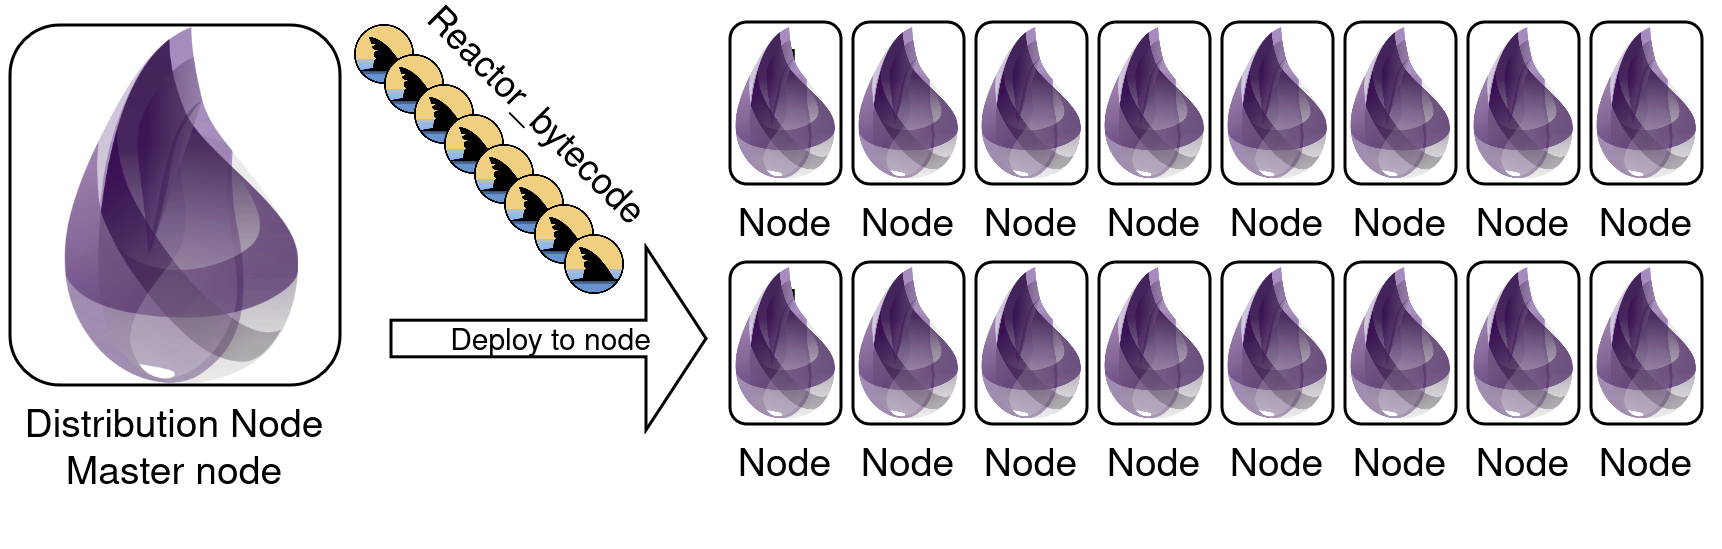
\includegraphics[width=\textwidth]{distribution300.drawio}
	\caption{Distributing reactor deployment on Elixir cluster}
	\label{fig:rdi}
\end{figure}  

Once the deployments are active each deployment will start sending messages towards the monitor of the cluster. The monitor is aware of the duration each single deployment uses to operate. Comparing the actual timing with the timings in the monitors directory we can asses about the individual deployments. For example if the actual timing is slower then the recorded timings in the monitor we might want to liberate more resources. The differences in timing are the starting poit of an investigation into what might cause this difference.

\section{Distributed environment}
We explain here in more detail the details of the system on which the Hvm is running..........?

\subsection{Shared-nothing architecture}
To organize the distribution of the Haai virtual machine we have opted for a shared-nothing architecture. (\cite{DBLP:journals/debu/Stonebraker86}) This allows us to build the cluster with the following characteristics, suitable for our research in distributing the reactive language Haai.
\begin{description}
	\item[Independent Nodes] Each node can execute its own specific code and perform computations independently since no memory, storage or processing power is shared.
	\item[No shared state] Each node manages its state independently. Cluster communication between nodes is done with messages. we use Erlang distributed mechanisms in the implementation.
	\item[Horizontal scalability] Shared-nothing architectures are highly scalable horizontally, this makes it straightforward to add or remove nodes from the cluster. It allows us to run clusters of all sizes. Practically the cluster size will be bound to the available hardware.
	\item[Fault isolation] Faults or failures in one node do not affect the operation of other nodes in the system. We can monitor node failure with Erlang distributed mechanisms and act accordingly. 
	\item[Flexibility and Modularity] Changes to one node do not impact the operation of other nodes, allowing for maintenance, upgrades, and system evolution of the cluster.` 
\end{description}

\subsection{Erlang virtual machine}

We implemented the shared-nothing architecture in Elixir a functional, concurrent, and fault-tolerant programming language built on the Erlang Virtual Machine (BEAM). The Erlang Virtual Machine provides a robust platform due to several key features and design principles:
\begin{description}
	\item[Concurrency model] Erlang has a lightweight concurrency model which is based on actor-like processes. Since each process runs independently and can communicate with other processes trough message passing the Erlang virtual machine is inherently decentralized by design.
	\item[Fault tolerance] The BEAM VM provides mechanisms for process supervision, fault isolation, and hot code swapping, allowing systems to recover from failures without affecting the overall operation of the cluster.
	\item[Distribution transparency] Erlang's distribution features enable processes to communicate effortlessly across network boundaries. Within an Erlang cluster, nodes can seamlessly interact through remote procedure calls (RPCs) and message passing. Different types of distribution models can be build on the Erlang platform.
	\item[Scalability] Horizontal scaling or adding nodes to a cluster is straightforward. This makes it easy to scale clusters to need.
	\item[Tooling] Common tasks are simplified thanks to a comprehensive tool set. tools like the Mix build tool and the OTP framework are core tools used in the implementation of the distributed Haai cluster.
\end{description}

The example program is explained in more detail in the use case chapter. The same program or reactor can be run many times. The distributed setup we make exists out of a number of elixir nodes that all send there messages to one sound server. The bigger the distributed network is the more messages that are send to the sound server. The sound server it self has virtually no limit to receive messages. The main parts of the distribution are taken care of by the underlying Beam virtual machine. One main reason to develop the Hvm on this platform is to be able to distribute in a solid and proven way.  

\subsection{Actor model}
The actor system in Erlang implements the processes actor model. (\cite{de_koster_43_2016}) These actors are modeled as processes and can define there receive primitive to specify what messages it responds to. Thanks to the isolated turn principle the actor model guarantees to be free of data races and deadlocks by design.
In Erlang actors are typically used when you need to encapsulate state and behavior within a single unit of computation., actors are spawned using constructs like GenServer, Task, or Agent within a single node. All actors communicate with each other using message passing within the same node. One can use these actors for modeling concurrent and stateful components in an application.

\subsection{Distributed Erlang mechanisms}
Distributed Erlang mechanisms come into play when you need to communicate between actors residing on different nodes within a cluster.
Nodes communicate with each other using distributed Erlang protocols, allowing actors on different nodes to exchange messages. Distributed Erlang mechanisms provide fault tolerance, distribution transparency, and location transparency across the cluster. 

Distributed Erlang provides location transparency, allowing actors to communicate regardless of their physical location within the cluster. This transparency hides the underlying network details, promoting loose coupling (\cite{DBLP:conf/tools/CarretonMCM10}) between nodes and actors. Actors on different nodes can interact seamlessly through message passing, without needing to be aware of the specific nodes they are communicating with. Loose coupling in distributed Erlang enables the system to scale horizontally by adding or removing nodes without significantly impacting the overall architecture.

\chapter{Evaluation} \label{sec:evaluation}


\section{Evaluating the distribution model}

The master-slave model used in our distribution works well. We have a cluster of actors, with basically two different types of actors. The master actor and the slave actors. This model allows us to handle issues with the slaves in a timely fashion by reacting as soon as inconsistencies between the recorded and live timings exist in the cluster monitor. The challenges mentioned in section \ref{sec:drp} are controllable within this model. We can guarantee glitch freedom on the individual basis of a node. Each individual node guarantees glitch freedom and in our master-slave model where we have no values exchanged between the nodes we do not expect other sources of inconsistency. 

The individual nature of the nodes in the cluster guarantees that when one node goes down no other nodes are impacted by this. The monitor of the cluster can based on timing measurements decide on a tactic to solve the possible failure of a node. For example if a node actual time is not updating the node must have trouble. we can spin up a node to replicate or solve the actual problem the initial node is having. the organization of the applicable tactics the monitor can perform are not part of this work but provide ... for future work. 

Working with the cluster monitor and the individual nodes requires only a small amount of network traffic. The cluster monitor will receive one message on a per duration time tempo for the deployed reactor. In the case of an issue the second process of the cluster monitor needs only to communicate with one single (new) node. The shared nothing architecture makes it simple to add or remove individual nodes.

The number of nodes that simulate the cluster can easily be a tenfold. The reactors itself have a very light computational cost existing out of some basic arithmetic operations. One Elixir node would consumes about 90MB of memory and virtually no processor time when idle and about 3\% when performing the calculation. This allowed to simulate a cluster on one machine with up to a hundred nodes. 

The next section explains the Distributed reactive melody generator (drmg) figuring here as a stand in for the cluster monitor. The drmg receives for each deployment a message on a predefined tempo per deployment. What we do here is having a synthesizer play a note equal to the duration of the deployment tempo for each node. All these single notes come together to form a melody. 
  

\section{Distributed reactive melody generator}
The distributed Haai cluster, existing out of many distributed reactors provides the sink values form the reactors as values inserted into OSC messages (\cite{schmeder2010best}) that are send to a sound server to trigger the synthesis of some sound. It is the reactors that, by reacting on incoming streams of data, produce the values that result in a rhythmical flow of OSC messages to the sound server. 

\begin{figure}[h]
	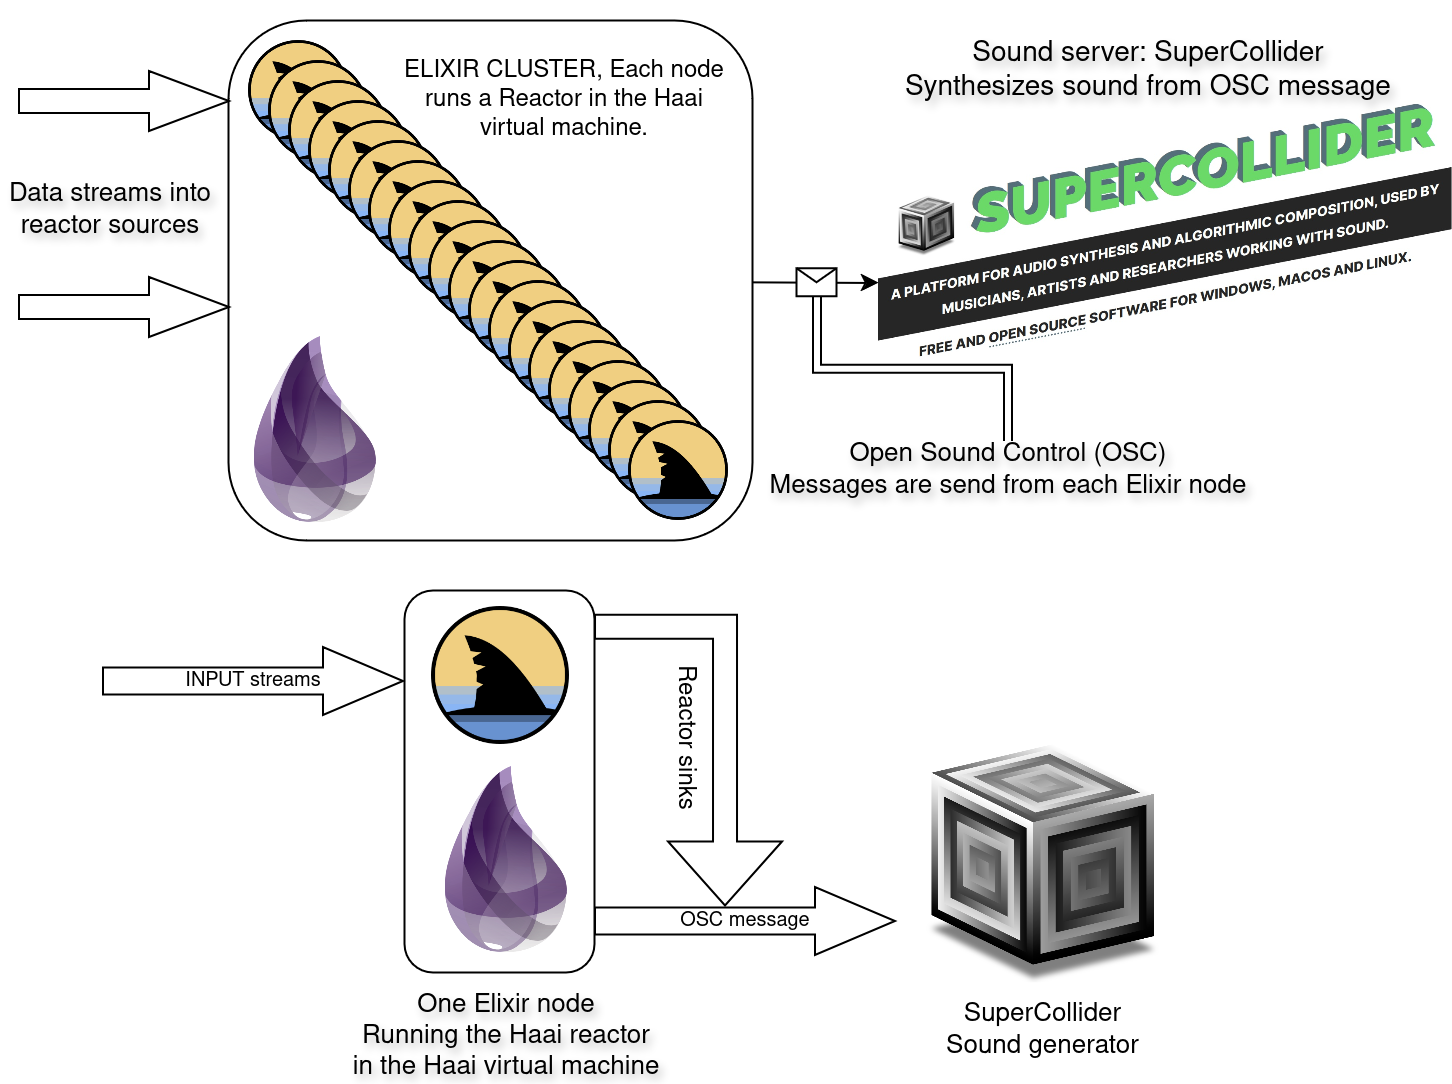
\includegraphics[width=\textwidth]{drmg200.drawio}
	\caption{Distriuted Reactive Melody Generator}
	\label{fig:drmg}
\end{figure}
 
The flow of rhythmical messages is related to the duration of each sound. That same duration that makes the sound disappear after it was started determines the iteration speed for the reactor or program that runs on each individual node. Each reactor iterates over and over but each iteration has a defined duration, this duration is virtually equal to the duration for a sound calculated by the reactor. A reactor will calculate the new values, sleep for the calculated duration and then provide the new values in the sink. At this point the Hvm calls a function that it was given to handle the sink values. For this use case that function constructs the message and sends it to the sound server that propagates it to the requested synthesizer. 

\subsection{Sound server}
The synthesizer that produces the sound is a Synthdef (the definition of a synthesizer) inside the sound server named Supercollider. Supercollider is an open-source platform for audio synthesis and algorithmic composition. Developed by James McCartney in the late 1990s (\cite{scBook}), it has since become a powerful tool in the fields of music technology, computer music, and sound art. Supercollider provides a flexible and expressive environment for creating and manipulating sound in real-time, making it an invaluable resource for both research and artistic exploration. Some main features of Supercollider include:

\begin{description}
	\item[Audio Synthesis] Supercollider offers a wide range of synthesis techniques, including additive, subtractive, granular, and physical modeling synthesis. Users can create complex sounds by combining these techniques and modulating parameters in real-time.
	\item[Real-time Processing] One of Supercollider's key strengths is its ability to process audio in real-time. This makes it suitable for live performances, interactive installations, and other time-sensitive applications.
	\item[Algorithmic Composition] Supercollider provides tools for generating music algorithmically, allowing users to create compositions based on mathematical algorithms, rulesets, or generative processes.
	\item[Integration with External Hardware] Supercollider can interface with external MIDI controllers, audio interfaces, and other hardware devices, enabling users to incorporate physical instruments and sensors into their sound projects.
	\item[Community and Documentation] Supercollider has a vibrant online community of users who share code, tutorials, and resources. Additionally, comprehensive documentation is available, including tutorials, reference guides, and examples to help users learn and master the software.
	
	
\end{description}

SuperCollider has been and still is actively used in academia for many purposes, for example:
\begin{description}
	\item[Research in Music Technology] Digital signal processing, human-computer interaction, and machine learning for music. Researchers leverage its flexibility and programmability to prototype new algorithms, experiment with novel synthesis techniques, and investigate the perceptual and cognitive aspects of sound.
	\item[Composition and Sound Design] Supercollider is used to create innovative works that push the boundaries of traditional music and sound art. Its ability to generate complex and evolving textures, as well as its support for algorithmic composition, makes it a valuable tool for exploring new sonic territories.
	\item[Teaching and Learning] Supercollider is increasingly incorporated into music technology and computer music curricula at universities and colleges worldwide. It provides students with hands-on experience in sound synthesis, programming, and digital audio processing.

\end{description} 
\subsection{Sound server communication}
The communication between the nodes in the Elixir cluster and the sound server is done over the network using the UDP network protocol. The sound server can handle a virtual unlimited amount of messages, but is practically bounded to the udp buffer size on the actual machine that runs the sound server. As such the Elixir cluster of reactors can be of any feasible size and the sound server will respond on any number of messages by synthesizing the requested sound. 

\subsection{Musical values}
The reactor or program that runs on all nodes in the cluster does for each note the following. It calculates two values given two input streams of numbers. The first source is a stream of base frequencies, represented as a float number, the second source is again a stream of numbers representing a tempo in beats per minute (bpm)

\subsubsection*{Consonant notes}
Consonant notes sound harmonious when played together. consonance can be expressed as a ratio between two notes or frequencies. Ratios like the perfect fifth (frequency ratio of 3:2) and the major third (frequency ratio of 5:4) are very commonly used ratios in a musical setting. One of the two reactors in the main program used for this use case calculates such a note for a given base note, both are expressed in there actual frequency represented as a float number.

\subsubsection*{Tempo}
We can express the speed of a musical note progression in beats per minute (bpm). From that number we can then calculate the duration of individual notes in the musical performance. 

We calculate the time in milliseconds. Since one minute is 60000 milliseconds one can calculate the length of a quarter note with \(q = \frac{60000}{bpm}\) with the assumption that we use a 4/4 time signature. From the length of the quarter note it is easy to find other durations. For example, the duration of a halve note is double that of a quarter note or the duration of a eight note is half the time of a quarter note.

One of the two reactors in the main program used for this use case calculates exactly that, the length for a quarter note and improvises a deviser or multiplier to produce some duration. 

%\backmatter
\chapter{Conclusion}
In conclusion, this thesis presents a comprehensive exploration of distributing reactive programming within the framework of the purely functional reactive language Haai. By addressing critical challenges such as consistency, fault tolerance, and communication overhead, we developed a system capable of efficiently scaling across distributed environments. The adoption of a shared-nothing architecture, coupled with the implementation of an Erlang cluster, facilitated the creation of a robust and resilient reactive system. The Haai virtual machine (Hvm) demonstrated effective management of distributed reactive programs, leveraging native reactors and ensuring glitch-free operation. This research contributes to the broader understanding of distributed reactive programming and provides a solid foundation for future developments in building scalable, fault-tolerant reactive systems.


\section{Further work}
The cluster monitor would be an addition to this work, different distribution models could be explored towards models that do comunicate 

Further work can be organized to explore different distribution models on the same Elixir set of nodes. Where all nodes did react independently of each other, in future work communication between nodes can be explored and more different programs or reactors can be setup and linked together...
Study glitch avoidance 

\printbibliography
\end{document}
